\section{Introduction}
\pgfdeclareimage[width=1.0\paperwidth]{header-image}{header_images/kata_tjuta}

\begin{frame}
    \frametitle{It burns where it rains}
    \framesubtitle{Uni-modal relationship with moisture}

    \foreach \x in {0, 1, 2, 3, 4, 5, 6, 7, 8, 9, 10} {
        \only<\x> {
        \begin{textblock*}{10cm}(0cm,1.5cm)
            \includegraphics[width=13.0cm]{images/unimodal/p\x.png}%images/unimodal/p\x.png}
    \end{textblock*}
    }}
    %Make clear we are talking about burnt area
\end{frame}

\begin{frame}<1-3>[label = intro]
    \frametitle{What else controls fire?}
    \framesubtitle{Is it Ignitions? Is it people?}
	\begin{itemize}
		\visible<2-> {\item Fire-vegetation models incorporate ignition schemes}
		\visible<3-> {\item Schemes often include human and lightning caused ignitions}
		\visible<4-> {\item All models with human-caused igntions show increased burnt area with people}
		\visible<5-> {\item Little effort placed in anthropagenic fire supression}
	\end{itemize}

\end{frame}

\begin{frame}
    \frametitle{What else controls fire?}
    \framesubtitle{Is it Ignitions? Is it people?}
    FireMIP slide from Stijn
    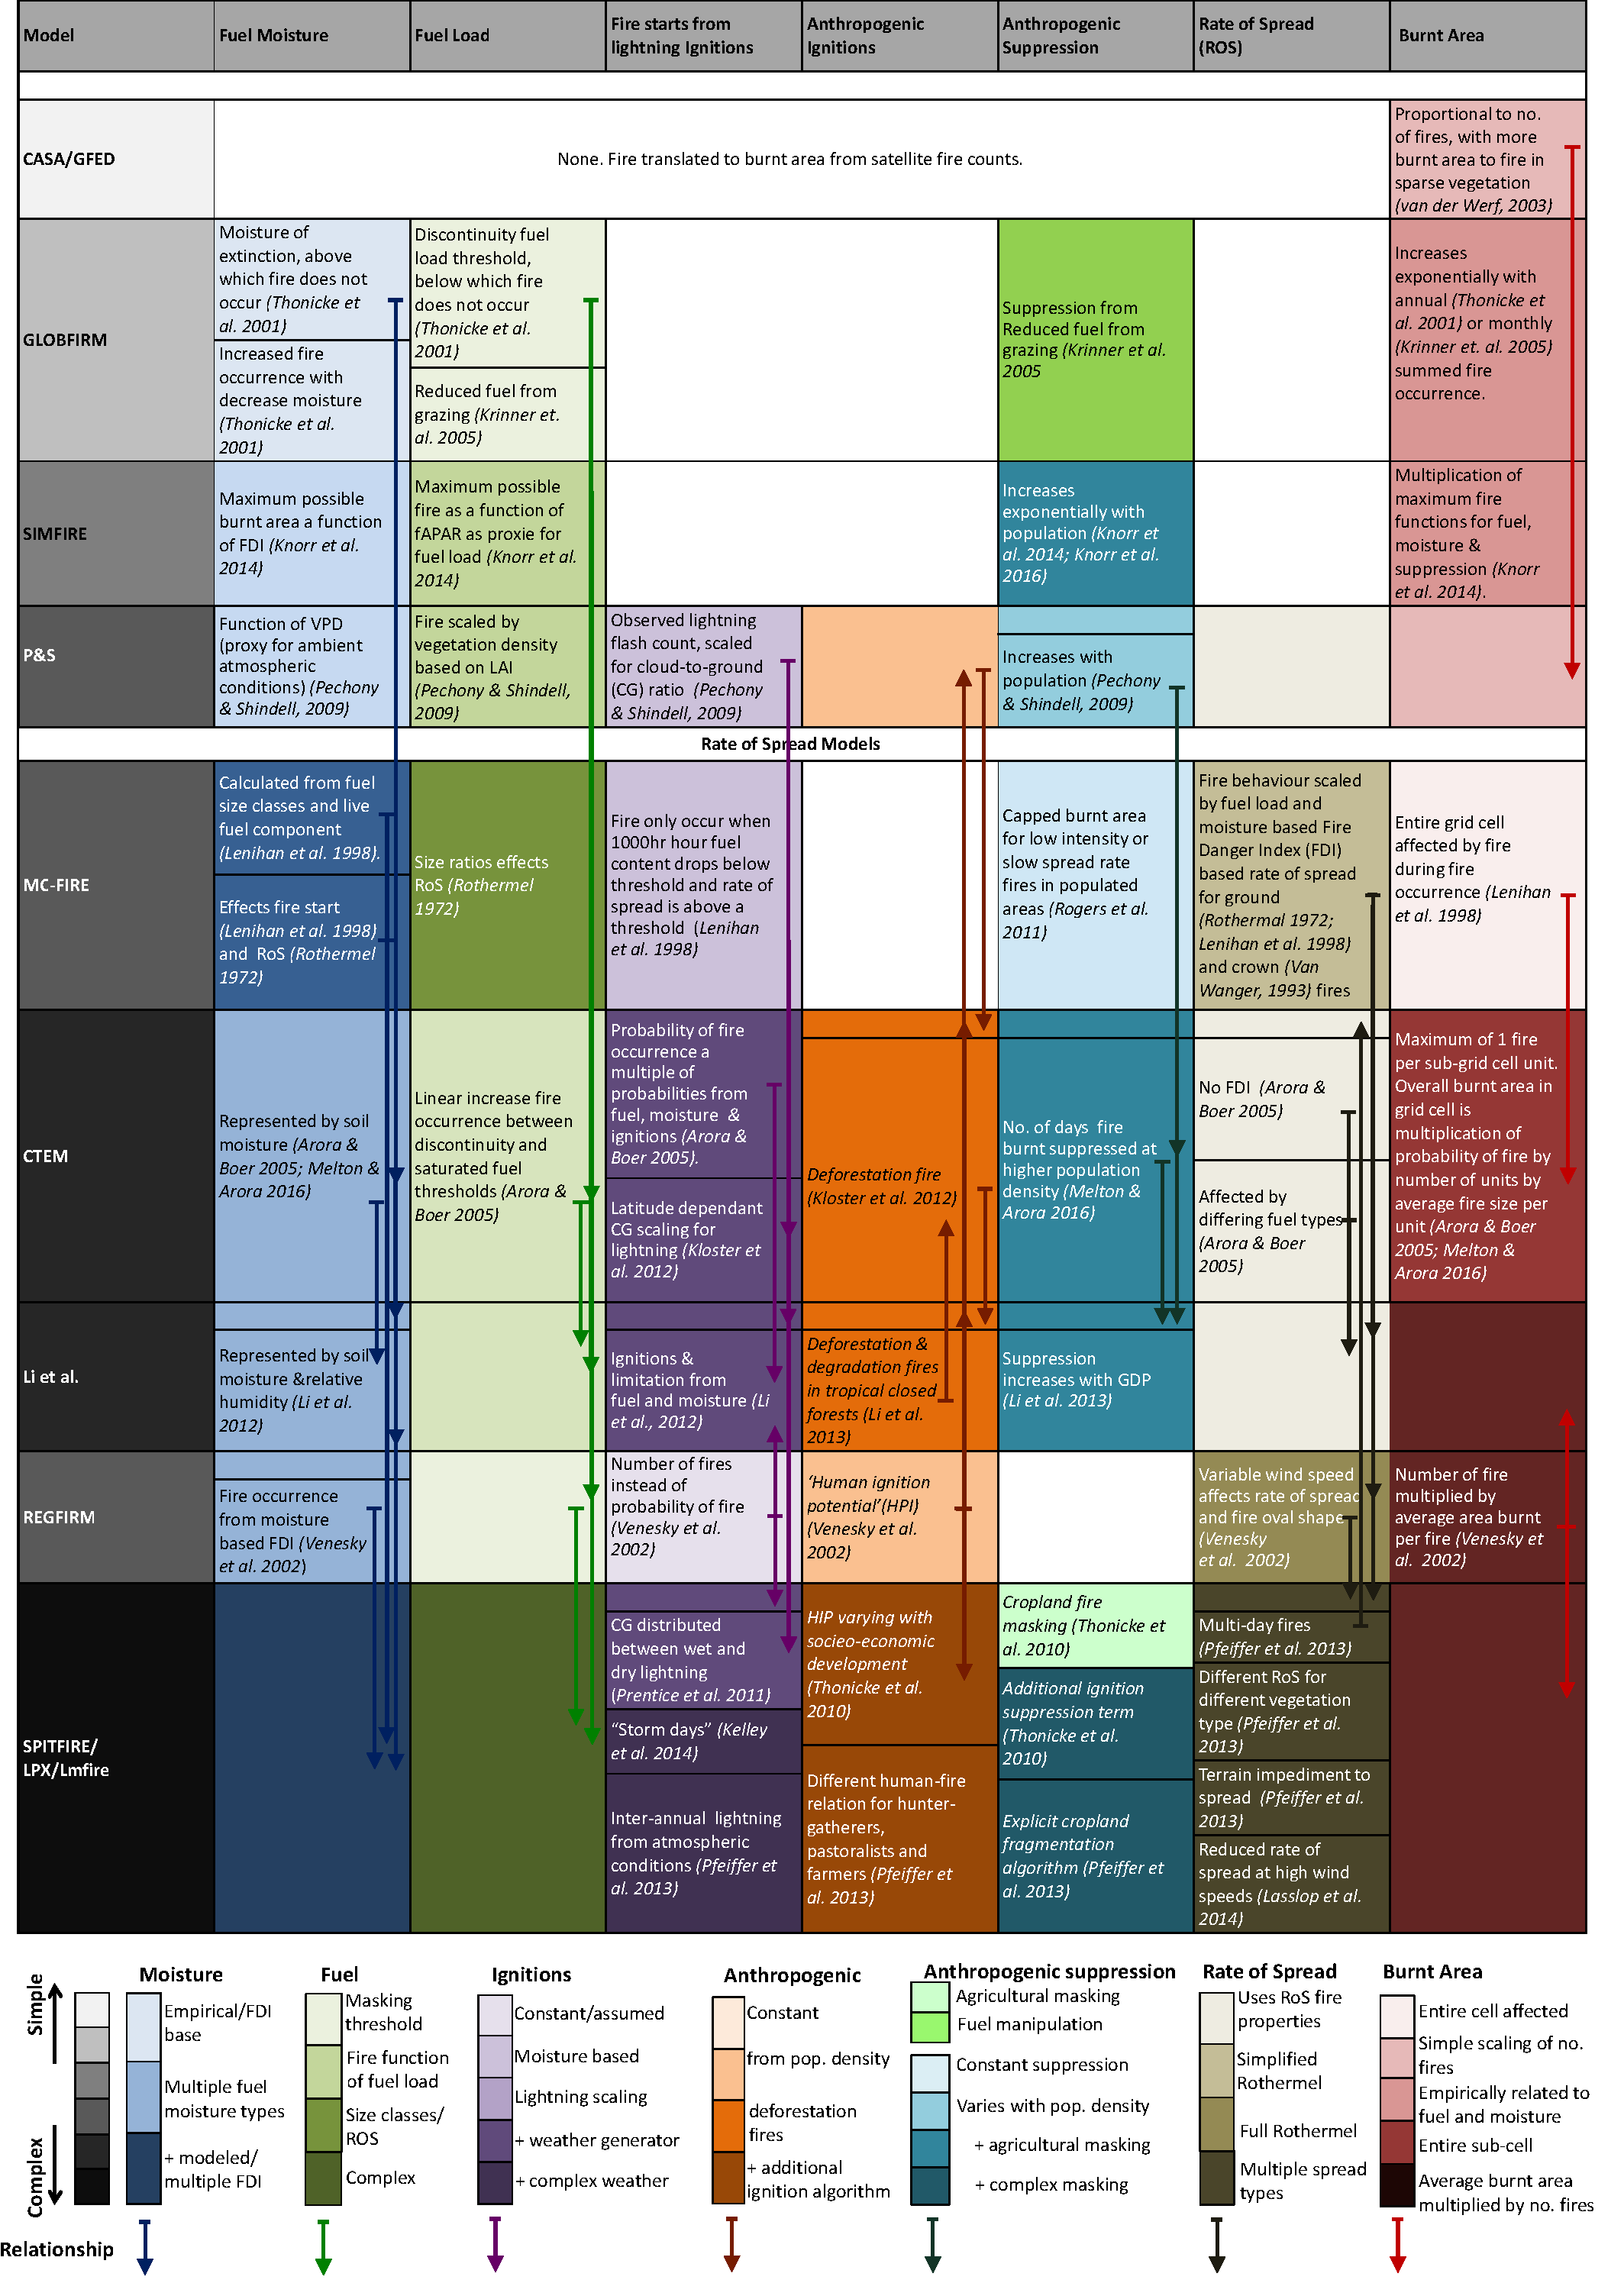
\includegraphics[width=3cm]{images/Table1.pdf}%images/unimodal/p\x.png}
\end{frame}

\againframe<3-4>{intro}

\begin{frame}
    \frametitle{What else controls fire?}
    \framesubtitle{Is it Ignitions? Is it people?}
    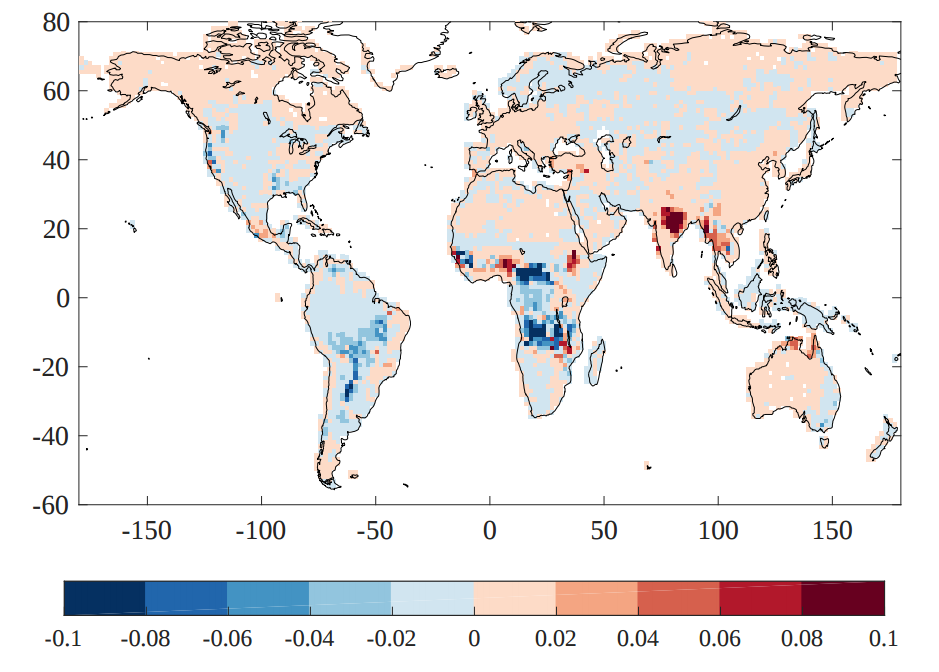
\includegraphics[width=9.0cm]{images/INFERNO}%images/unimodal/p\x.png}
	%Inferno plot
\end{frame}

\againframe<4->{intro}



\begin{frame}
    \frametitle{What else controls fire?}
    \framesubtitle{Fire-limitation framework}
	\begin{itemize}
		\visible<2-> {\item map the limitation and sensitivity of burnt area to}
        \begin{itemize}
            \visible<3-> {\item Fuel discontinuity}
            \visible<4-> {\item Fuel moisture and atmospheric drying potential}
            \visible<5-> {\item lightning and human ignitions}
            \visible<6-> {\item land use and human supression}
        \end{itemize}
		\visible<7-> {\item Controls are described from remote sensed and meteorological observations}
		\visible<8-> {\item optimized againstburnt area observations}
	\end{itemize}
\end{frame}
